\section{Gram-Schmidt as a Deformation Retract}
\label{s:deformation_retract}
\begin{definition}[Gram-Schmidt orthogonalization]
The Gram-Schmidt orthogonalization ($GS$) of a matrix $A$ of the form $A \Let (v_1, v_2, \ldots , v_n)$ where $v_i \in \R[n]$ are the column vectors of $A$ is given by,
$GS: GL_n(\R) \times [0, \frac{1}{2}] \mapsto GL_n(\R)$ is defined as,
$$GS(A, t) \Let \bigl((1-2t)v_1 + 2tu_1, \ldots, (1-2t)v_n + 2tu_n\bigr),$$ where each $u_i$ is defined as
$$u_1 = v_1,$$
$$u_2 = v_2 - \frac{\innerprod{u_1, v_2}}{\norm{u_1}}u_1,$$
$$u_n = v_n - \sum_{k=1}^{n-1}\frac{\innerprod{u_k, v_n}}{\norm{u_k}}u_k.$$
\end{definition}
Since Gram-Schmidt orthogonalization generates an orthogonal set of $n$ vectors from a linearly independent set of $n$ vectors, the image of $A$ is equal to image of $GS(A, t)$ implying $GS(A, t)$ attains full rank for all $t$. Hence for all $t \in [0, \frac{1}{2}]$, $GS(A,t) \in GL_n(\R).$ 
\begin{definition}[Normalization map]
The normalization map for a matrix $A$ as defined above, given by $N: GL_n(\R) \times [\frac{1}{2}, 1] \mapsto GL_n(\R)$ defined by:
$$N(A,t) \Let \bigl(v_1(\frac{2t-1}{\norm{v_1}} + 2 - 2t), \ldots , v_n(\frac{2t-1}{\norm{v_n}} + 2 - 2t)\bigr).$$
\end{definition}
The map $N$ is designed such that $N(A,\frac{1}{2}) = A$ and $N(A, 1) = \bigl(\frac{v1}{\norm{v1}}, \ldots ,\frac{v_n}{\norm{v_n}}\bigr)$. We must check that for all $t \in [\frac{1}{2},1]$, $N(A,t) \in GL_n(\R)$. Computing the determinant, given by
$$\mathrm{det}\bigl(N(A,t)\bigr) = \mathrm{det}(A)\prod_{i=1}^{n}(\frac{2t-1}{\norm{v_i}} + 2 - 2t).$$
We must check that $\frac{2t-1}{\norm{v_i}} + 2 - 2t \neq 0$ $\forall$ $1\leq i \leq n$. Assume this is true for some $i$. Then,
$$\frac{2t-1}{\norm{v_i}} + 2 - 2t = 0$$
$$\implies 2t - 1 = 2t\norm{v_i} - 2\norm{v_i}$$
$$\implies t = \frac{1 - 2\norm{v_i}}{2(1 - \norm{v_i})}.$$
Plotting the function $y = \frac{1-2x}{2(1-x)}$on a graphing-calculator (Desmos) shows that it has no solutions for $y \in [\frac{1}{2}, 1]$. Hence, we have shown a contradiction which implies that $\mathrm{det}\bigl(N(A,t)\bigr) \neq 0 \implies N(A,t) \in GL_n(\R)$ $\forall$ $t \in [\frac{1}{2},1].$ 

\begin{definition}[Gram-Schmidt orthonormalization]
Defining the Gram-Schmidt ortho-normalization (GSO), given by $GSO: GL_n(\R) \times [0,1] \mapsto GL_n(\R)$ and defined by
\[
    GSO(A,t) = 
\begin{cases}
    GS(A,t),& \text{if } t\in [0, \frac{1}{2})\\
    N(A,t),& \text{if } t\in [\frac{1}{2}, 1]
\end{cases}.
\]
This is well-defined since $GS(A,t)$ and $N(A,t)$ agree at $t=\frac{1}{2}$.
\end{definition}

\begin{theorem}
The $GSO$ as defined above is a strong deformation retraction of $GL_n(\R)$ into $O(n)$.
\end{theorem}
\emph{Proof}: Observe that $GSO(A,0) = A \in GL_n(\R).$ Next, $GSO(A,1)$ is a matrix with ortho-normal columns implying $GSO(A,1) \in O(n)$. Further, any element $A \in O(n)$ remains fixed since $\innerprod{u_k, v_i} = 0$ for all $1 \leq i \neq k \leq n$ and therefore, for all $t \in [0,\frac{1}{2}]$, we have $GS(A, t)=A$. For such a matrix,$N(A, t)=A$ for $t \in [\frac{1}{2},1]$ (As $\norm{v_i} = 1$ for all $1 \leq i \leq n)$. Thus, this is a strong deformation retraction. For the simple case of $n=1$, this deformation retraction can be visualized as given in Figure~\ref{fig:deform-retract}.
\begin{figure}[t]
  \centering
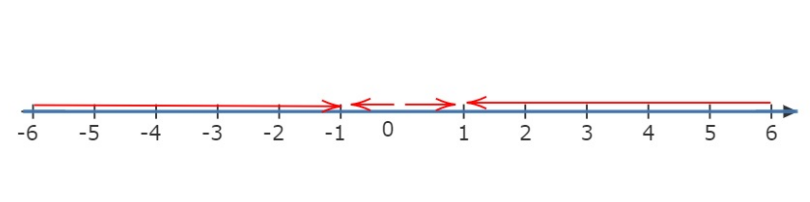
\includegraphics[width=10cm]{RealLine-deformation-retract.png}
\caption{Deformation retraction of $GL_1(\R)$ $\bigl((-\infty, 0)\cup (0, \infty)\bigr)$ to $O(1)$ $\bigl(\{-1, 1\}\bigr)$}
  \label{fig:deform-retract}
\end{figure}
